\subsection{Caches and Address Translation}
\label{sec:tlbs}

Modern system software relies on address translation (\S~\ref{sec:paging}).
This means that all the memory accesses issued by a CPU core use virtual
addresses, which must undergo translation. Caches must know the physical
address for a memory access, to handle aliasing (multiple virtual addresses
pointing to the same physical address) correctly. However, address translation
requires up to 20 memory accesses (see Figure~\ref{fig:vmx_paging}), so it is
impractical to perform a full address translation for every cache access.
Instead, address translation results are cached in the \textit{translation
look-aside buffer} (TLB).

Table~\ref{fig:tlb_timings} shows the levels of the TLB hierarchy. Recent
processors have separate L1 TLBs for instructions and data, and a shared L2
TLB. Each core has its own TLBs (see Figure~\ref{fig:cpu_core}). When a virtual
address is not contained in a core's TLB, the \textit{Page Miss Handler} (PMH)
performs a \textit{page walk} (page table / EPT traversal) to translate the
virtual address, and the result is stored in the TLB.

\begin{table}[hbt]
  \centering
  \begin{tabular}{| l | r | r |}
  \hline
  \textbf{Memory} & \textbf{Entries} & \textbf{Access Time}\\
  \hline
  L1 I-TLB & 128 + 8 = 136 & 1 cycle \\
  \hline
  L1 D-TLB & 64 + 32 + 4 = 100 & 1 cycle \\
  \hline
  L2 TLB & 1536 + 8 = 1544 & 7 cycles \\
  \hline
  Page Tables & $2^{36} \approx 6 \cdot 10^{10} $ & 18 cycles - 200ms \\
  \hline
  \end{tabular}
  \caption{
    Approximate sizes and access times for each level in the TLB hierarchy,
    from \cite{7zip2014haswell}.
  }
  \label{fig:tlb_timings}
\end{table}

% Caching Translations in TLBs: SDM S 4.10.2.2
% Caches for Paging Structures: SDM S 4.10.3.1

In the Intel architecture, the PMH is implemented in hardware, so the TLB is
never directly exposed to software and its implementation details are not
documented.  The SDM does state that each TLB entry contains the physical
address associated with a virtual address, and the metadata needed to resolve a
memory access. For example, the processor needs to check the writable (W) flag
on every write, and issue a General Protection fault (\#GP) if the write
targets a read-only page.  Therefore, the TLB entry for each virtual address
caches the logical-and of all the relevant W flags in the page table structures
leading up to the page.

The TLB is transparent to application software. However, kernels and
hypervisors must make sure that the TLBs do not get out of sync with the page
tables and EPTs. When changing a page table or EPT, the system software must
use the INVLPG instruction to invalidate any TLB entries for the virtual
address whose translation changed. Some instructions \textit{flush the TLBs},
meaning that they invalidate all the TLB entries, as a side-effect.

% Large Page Size Considerations: SDM S 11.11.9

TLB entries also cache the desired caching behavior (\S~\ref{sec:memory_io})
for their pages. This requires system software to flush the corresponding TLB
entries when changing MTRRs or page table entries. In return, the processor
only needs to compute the desired caching behavior during a TLB miss, as
opposed to computing the caching behavior on every memory access.

% Propagation of Paging-Structure Changes to Multiple Processors: SDM S 4.10.5

The TLB is not covered by the cache coherence mechanism described in
\S~\ref{sec:cache_coherence}. Therefore, when modifying a page table or EPT on
a multi-core / multi-processor system, the system software is responsible for
performing a \textit{TLB shootdown}, which consists of stopping all the logical
processors that use the page table / EPT about to be changed, performing the
changes, executing TLB-invalidating instructions on the stopped logical
processors, and then resuming execution on the stopped logical processors.

Address translation constrains the L1 cache design. On Intel processors, the
set index in an L1 cache only uses the address bits that are not impacted by
address translation, so that the L1 set lookup can be done in parallel with the
TLB lookup. This is critical for achieving a low latency when both the L1 TLB
and the L1 cache are hit.

Given a page size $P = 2^{p}$ bytes, the requirement
above translates to $l + s \le p$. In the Intel architecture, $p = 12$, and all
recent processors have 64-byte cache lines ($l = 6$) and 64 sets ($s = 6$) in
the L1 caches, as shown in Figure~\ref{fig:caching_and_paging}.
The L2 and L3 caches are only accessed if the L1 misses, so the physical
address for the memory access is known at that time, and can be used for
indexing.

\begin{figure}[hbt]
  \centering
  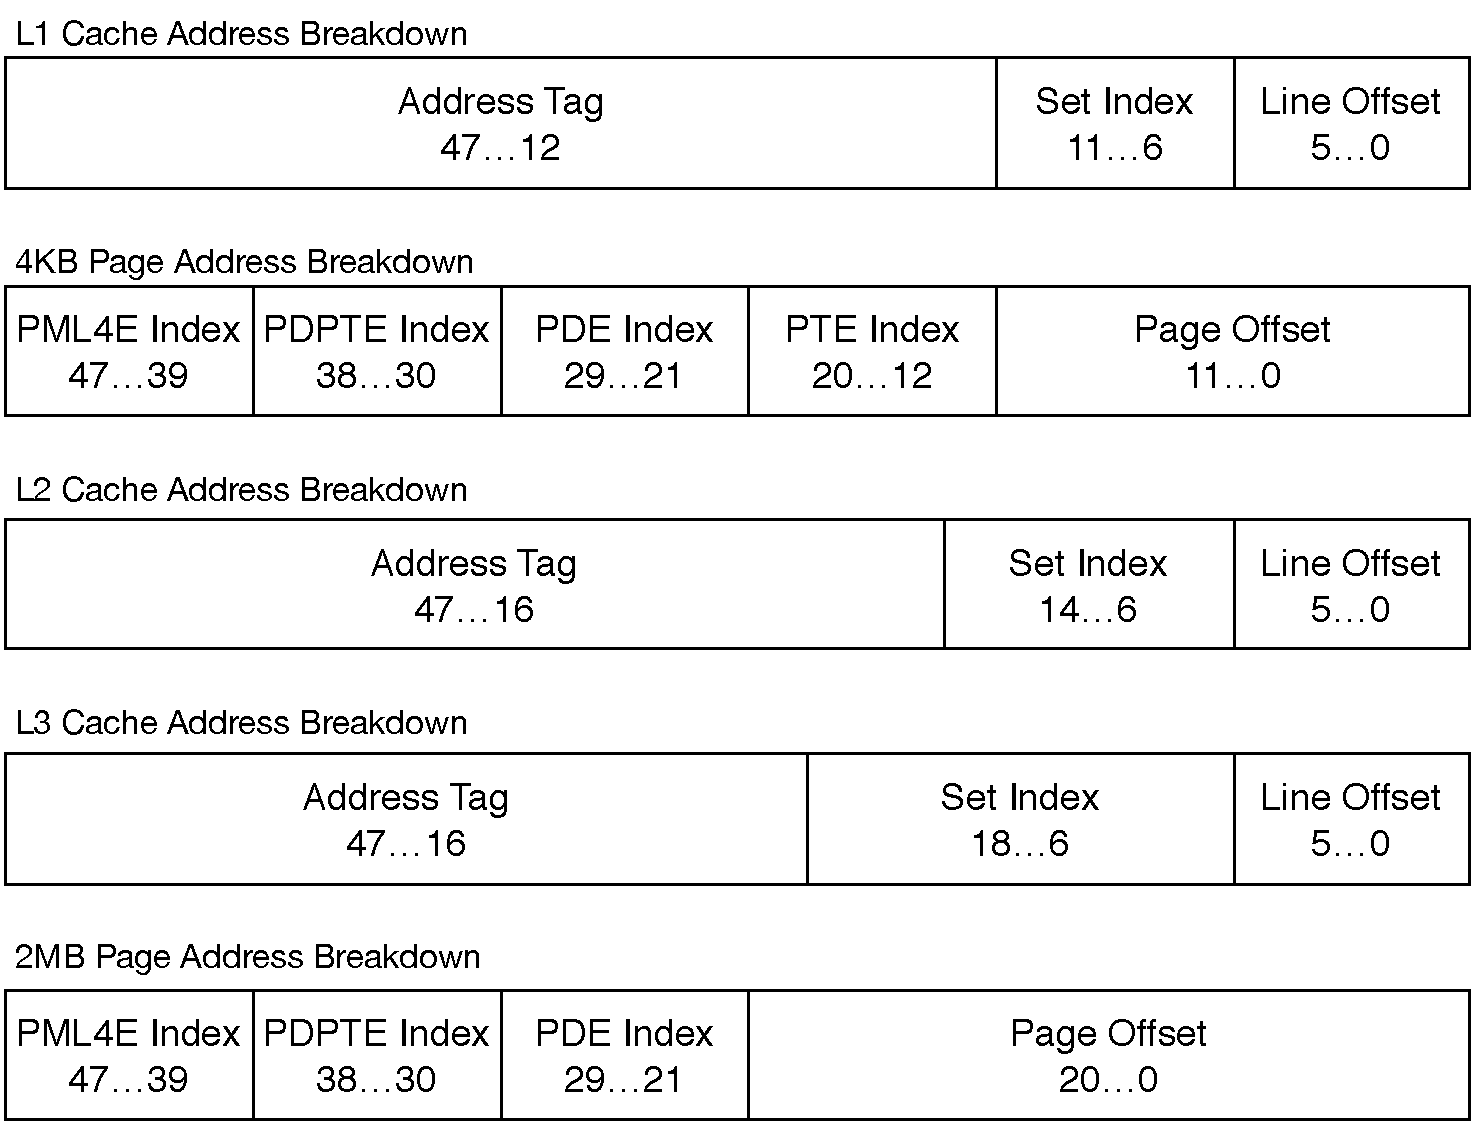
\includegraphics[width=87mm]{figures/caching_and_paging.pdf}
  \caption{
    Virtual addresses from the perspective of cache lookup and address
    translation. The bits used for the L1 set index and line offset are not
    changed by address translation, so the page tables do not impact L1 cache
    placement. Page tables do impact L2 and L3 cache placement. Using large
    pages (2~MB or 1~GB) makes cache placement independent of page tables.
  }
  \label{fig:caching_and_paging}
\end{figure}
